\chapter{Method}
\label{chap:method}

% In this chapter, we discuss the methodology of the thesis. We motivate and specify the research question, state the hypothesis and the specify how we test it.

% Methodology

% what do we want to measure? The effects of tokenization over the languages, focus on the differences the methods make on low resource vs high resource and how this translates to downstream tasks.b

% - data sampling
%     - !! do data hodně vysvětlit, že u toknizerů používáme různá alpha ale u pretrainingu ne.

% - introduce the metrics
%     - obecně naše metriky předpokládají nějaký předem daný vocabulary budget, který chceme spravedlivě rozdělit
%     - CPT, AR, JSD
%         - k AR metrice: je to samozřejmě závislý na vocab size, ale měl bych to poznamenat
%         - výhoda AR oproti CPT - u čínštiny započítává jednotlivé znaky, což by u CPT nebylo vidět

%         - k JSD metrice: není zřejmé jestli chceme vyšší overlap nebo nižší

%     - interpretation of the metrics - CPT, AR high good, JSD not sure
%     - also mention UNK and alphabet size
% - kinds of experiments
%     - tokenizers only
%         - eg: training data size, alphabet size, data imbalance
%     - tokenizers + MLM training
%         - eg: Huggingface tokenizers, replications
    
% - introduce the evaluation procedure
%     - intrinsic evaluation
%         - overall metrics - why macro average over languages
%             - how to average JSD - all pairs
%         - per language metrics - why delta from some baseline, metrics are different for different languages so we need to normalize
%     - extrinsic evaluation
%         - in-language / cross-language
%             - overall - why macroaverage, per-language, how to do per-language in cross-lingual where there are pairs (we focus on target results)
%             - seeds, averaging, bootstrapping
            %     - on how to compute significance for the cross-lingual tasks
            %         - we want to compare the average over languages
            %         - we can use bootstrapping to compute the confidence intervals
            %             - for each language select a random seed and compute the average over these seeds
            %             - sample many times and compute the confidence intervals
%         - probing vs finetuningn
%             - vysvětlit proč jsou všechny experimenty probing a jak se to liší a proč jsme to vybrali
%         - tasks NLI, NER, POS tagging, ...
%     - correlation between intrinsic and extrinsic
%         - how to compute the correlation
%         - míra korelace závisí na tom, jak moc se liší experimenty. Když porovnáváme jen stejné experimenty, pak nám vyjde nízká

% \textbf{Q1:} How do subword tokenizers differ in overlap and allocation of learned vocabularies?
% \textbf{Q2:} Which properties of multilingual tokenizers affect the language model representation quality?
% \textbf{Q3:} What is the reason that the standard tokenizer training method does not work well in the multilingual setting? 
% \textbf{Q4:} What is the effect of using the reproduced methods on the representation of low-resource languages? And
% \textbf{Q5:} How do the reproduced methods compare to the standard method of training the tokenizer on balanced and unbalanced joint corpus?


In this chapter, we introduce the methodology for experiments conducted in this thesis. We introduce the important data sampling method utilized in \citet{devlin_bert_2019,conneau_unsupervised_2020} we use frequently for our experiments.
Then we introduce our proposed metrics for measuring the \textit{vocabulary allocation} and \textit{vocabulary overlap} of a tokenizer. 
We introduce the types of experiments we will conduct. 
\tomaszrep{Namely}{Overall,} we will train different tokenizers and evaluate them against our metrics.
\tomaszrep{Moreover,}{Subsequently,} we will also use the tokenizers to train masked language models to verify that our metrics are useful for assessing the tokenizer quality for use in language models. We will also describe in detail the evaluation procedures and all evaluation settings and tasks. 

% \xxx{TODO - WIP}
% In this chapter, we explain the methodology for experiments conducted in this thesis. We answer our research questions stated in the \autoref{chap:introduction} in the following manner. In the \autoref{sec:tokenizer_metrics}, we introduce metrics for measuring the quality of tokenizers. We use these metrics to investigate the differences between tokenizers (\textbf{Q1}, ). We then validate the usefulness of our metrics by training masked language models using the tokenizers and evaluating them on a set of downstream tasks to see whether are our metrics good predictors of the model performance. (\textbf{Q2}). Then we use our metrics on a more granular level and investigate the differences 


% For all experiments we use the CC100 dataset used in \citet{conneau_unsupervised_2020}. Using the data we create multilingual vocabularies with the same size of 120K unique tokens using different methods. We use intrinsic evaluation framework from \citet{limisiewicz_tokenization_2023} to evaluate the tokenizers. Then we use the tokenizers to train multilingual masked language models on the same data and evaluate them on the same set of downstream tasks. We compare the results of the intrinsic and extrinsic evaluation to see if the improvements in the intrinsic evaluation translate to improvements in the downstream tasks.

% In this thesis, we investigate the effect of tokenizer properties on multilingual language models. We define metrics that measure the properties of the tokenizers and then we define the method by which we assess how these properties affect the performance of the language models. At the same time we want to improve the performance of the multilingual language model for the low-resource languages as this was shown to be a problem in previous work \cite{rust_how_2021}. Therefore we use the metrics we define to assess the methods proposed to solve this problem. Furthermore we propose methods to improve the performance of the language models and evaluate them using the same metrics.


\section{Data sampling}
\label{sec:data_sampling}

% This subset of CC100 is then used for further experiments with vocabulary creation that will be described in the following sections.
% \xxx{TODO: describe the resampling method, compare different alphas used in the literature}
% For pretraining the models and training the tokenizers we do not use the full 10\% of the data. Because the data is heavily skewed towards the high-resource languages. Instead, we further subsample the data, following \citet{conneau_unsupervised_2020-1} to balance the number of lines per language. This is a standard practice followed by multiple independent authors \xxx{cite}. The empirical probability of sampling a line from language $l$ is given by:

% In the following chapters, we will reference often the balancing factor $\alpha$, here we defin

As explained in the previous chapters \tomasz{refer to specific chapter}, the training data available for each language differs significantly in the total size (counted as the number of lines). For training the multilingual language model and associated tokenizer, it is generally advised to address this data imbalance by oversampling the languages with a low amount of data available (low-resource languages) and undersample the languages with high amounts of data (high-resource languages). One possible balancing procedure proposed by \citet{devlin_bert_2019,conneau_unsupervised_2020} is parametrized by the exponent $\alpha$ which we will now describe.
\tomaszrep{In the following chapters, we will reference often the balancing factor $\alpha$. 
If not mentioned otherwise, we consider data balance in the \textbf{tokenizer} training data (not pretraining data for the model) implied by sampling with the $\alpha$ parameter.}{[confusing, the second sentence is reiterated clearer at the end of the section.]}

We assume we have $N$ monolingual corpora $C_l$ with languages $l \in L$. Each corpus with the language $l \in L$ has a different number of lines $N_l = |C_l|$. Then, the probability of sampling a line from the concatenation of all corpora $\cup_{l \in L} C_l$ is:

\begin{equation}
    p(l) = \frac{N_l}{\sum_{l' \in L} N_{l'}}
\end{equation}

% Where $N_l$ is the number of lines in the dataset for language $l$.

To ensure that the low-resource languages are not underrepresented in the training data, we modify this probability distribution using an exponential smoothing parameter $\alpha$:

\begin{equation}
    p'(l) = \frac{p(l)^\alpha}{\sum_{l' \in L} p(l')^\alpha}
\end{equation}

For $\alpha = 0.0$ we get a uniform distribution over the languages, for $\alpha = 1.0$ we get the original distribution. 

For pretraining the language models, we use $\alpha = 0.3$ as suggested by \citet{conneau_unsupervised_2020-1}. For training the tokenizers, we always specify the alpha as a parameter of the tokenizer training procedure. 

\section{Tokenizer metrics}
\label{sec:tokenizer_metrics}

% \xxx{lets write the motivation here and maybe move it to the background section later}  

% - motivation: we want to evaluate the tokenizers before costly pretraining
% - by comparing the tokenizers we can select the best one for pretraining
% - we can also use the metrics to study the effect of the hyperparameters and other factors on the tokenizer
% - We use the metrics throughout the thesis to measure the tokenizers
% - We can measure how the tokenizer output differs between languages
%     - Explain how to measure individual languages with the same tokenizer. Metric may be a function of the tokenizer and language coded hold out data

% - Why do we want to measure the tokenizers?
%     - we want to select the best tokenizer for pretraining
%     - how do the tokenizers differ?
%         - overlap between languages - can be beneficial for some tasks (ner) but detrimental for others (pos)
%         - how much do they split words? (Rust)
%         - how much do they split sentences? (Limisiewicz)
%             - too much splitting - the model needs to learn to reconstruct words
%             - too little splitting - there is not enough examples for the model to learn from (but maybe this is not a problem for masked LM, only for machine translation)
%         - we can also measure the compatiblity of the segmentations (Maronikolakis)
%         - vocabulary capacity per language
%             - are the languages represented equally in the vocabulary?
%             - this is hard because some languages need more tokens than others (Chinese vs English)

% - how to measure tokenizers
%     - we want to measure the per-language and cross-lingual phenomena
%     - we therefore need to measure the tokenizers using language-coded data
%     - the basis for measurement will be the tokenization of the language-coded data and the empirical distribution of the tokens

%     - Average Rank - we want to measure how many tokens are used in the vocabulary - high frequency tokens are penalized because they move the average down
%         - another motivation - AR is similar to "the number of tokens needed to cover x% of the data" but it is non-parametric and includes the information about the distribution of the tokens
%     - Characters per Token - more characters = less ambiguity = better
%         - similar to word fertility, equivalent to tokens per sentence
%             - tokens per sentence used in Chung (they call it description length), Liang
%         - usable also in the langugaes without spaces
%     - of course both measures depend on the langugage

%     - interesting: ALP === entropy * avg_sequence_length

%     - overlap - what is the overlap between two languages
%         - we can look at the number of tokens that are shared between the languages but this is not that informative because these tokens might be very rare
%             - Wu and Dredze did this
%         - better is to look at the distributions of the tokens in each language and measure the similarity
%         - we can use the Jensen-Shannon divergence to measure the similarity of the distributions
%         - Chung used the Wasserstein distance but this is a distance function defined between probability distributions on a given metric space. (probability measures). We do not see how to interpret the token distribution as a probability measure and Chung does not discuss this

In this section we introduce the metrics that we use to evaluate the tokenizers. By measuring the tokenizers we would like to explore two questions. First, we would like to analyse how the tokenizers differ between each other. How granular is the segmentation given an example text? And how much are the tokens shared between the languages? Second, using the observed differences between tokenizers, we would like to analyse how they influence the multilingual language models, that are trained using the tokenizers. We will describe the methodology for measuring the influences in the following sections \xxx{ref}.

When assessing the multilingual tokenizers, we also want to focus not only on the overall properties but also investigate the quality of tokenization for the individual languages. This gives us a better understanding of the tokenizers and allows us to compare the tokenizers with each other given a target language. For this purpose, we will use monolingual evaluation corpora for each language. The metrics we define will be therefore functions of the tokenizer $\tau$ and the corpus $C_l$ with the selected language $l$. 

We introduce three metrics - average rank, characters per token and Jensen-Shannon divergence. The first two metrics aim to measure the "vocabulary allocation" of the tokenizer --- the degree to which is the given language represented in the vocabulary. The third metric measures the "vocabulary overlap" between a given pair of languages --- the degree of token sharing between two languages.

% Later, in \autoref{sec:metric_comparison}, we compare our metrics with the metrics used in the literature.

To define the metrics formally, we use the following notation \cite{zouhar_tokenization_2023}. Let $\Sigma$ be a set of characters we call the alphabet. In our context, the alphabet is the set of all valid Unicode characters. We call a string $\sigma \in \Sigma^*$ a line \tomasz{wait, what is $\Sigma^*$? How is it different from $\Sigma$?}. Finally, we call a multiset of lines $C_l = \{ \sigma_1, \ldots, \sigma_{N_l} \} \subset \Sigma^*$ a corpus of size $N_l$. The $l \in L$ denotes a language of the corpus from a set of languages $L$. Next, we denote the set $V_\tau \subset \Sigma^*$ as the vocabulary of a tokenizer $\tau$. The tokenizer $\tau: \Sigma^* \rightarrow V_\tau^*$ is a mapping from a line $\sigma \in \Sigma^*$ to a sequence of tokens $\tau(\sigma) \in V_\tau^*$. We denote the number of tokens in a sequence $s$ as $|s|$. Finally, we denote the number of occurrences of a token $v \in V_\tau$ in a corpus $C_l$ as $\textrm{cnt}(v, C_l)$.
\xxx{TODO: Check the notation}
% For each metric we will provide motivation and comparison with similar metrics used in the literature. 

% \xxx{mention the vocabulary allocation and vocabulary overlap}
\xxx{TODO: add UNK rate?!}

\subsection{Characters per token}

\begin{figure}[h]
    \centering
    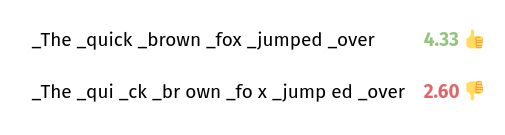
\includegraphics[width=0.6\textwidth]{img/temp/cpt_example.png}
    \caption{Example of CPT metric.}
    \label{fig:cpt_example}
\end{figure}

The first metric we propose is the average number of characters per token (CPT). The motivation for this metric is that we want to measure how granular the tokenization for a given language is. If the tokenizer splits the words into many tokens, the average number of characters per token will be low. On the other hand, if the tokenizer does not split the words, the average number of characters per token will be high. We hypothesize, that longer tokens are better for the language models, because they potentially carry more meaning. The extreme case of this metric is the character-level tokenization, where the average number of characters per token is 1. In this case the model would need to learn to reconstruct the words from the characters.

The metric is defined as follows. Given a tokenizer $\tau$ and a language corpus $C_l$, we first tokenize the corpus using the tokenizer $\tau$. Then we compute the average number of characters per token in the tokenized corpus:

\begin{equation}
    CPT(\tau, C_l) = \frac{\sum_{s \in C_l}|s|}{\sum_{s \in C_l}|\tau(s)|}
\end{equation}

where $|s|$ is the number of characters in the sentence $s \in C_l$ and $|\tau(s)|$ is the number of tokens in the tokenized sentence. The metric is illustrated in Figure \ref{fig:cpt_example}.

The CPT metric is connected to the \textit{average tokenized length} (or sequence length, or description length) metric used in \citet{chung_improving_2020,liang_xlm-v_2023}. 
These works suggest using the metric to compare whether one tokenizer splits a selected low-resource language into more tokens compared to another tokenizer. The average tokenized length is defined as the average number of tokens per sentence: 

\begin{equation}
\label{eq:tl_def}
    TL(\tau, C_l) = \frac{\sum_{s \in C_l}|\tau(s)|}{|C_l|}
\end{equation}

Where $C_l = {s_1, ..., s_{|C_l|}}$ from the language $l$ and $\tau$ is the tokenizer.

The tokenized length can be expressed as the product of the reciprocal of CPT metric and the average sentence length, which is corpus-specific and not dependent on the tokenizer:
\begin{equation}
\label{eq:tl}
    CPT(\tau, C_l)^{-1} \cdot \frac{\sum_{s \in C_l}|s|}{|C_l|} = \frac{\sum_{s \in C_l}|\tau(s)|}{\sum_{s \in C_l}|s|} \cdot \frac{\sum_{s \in C_l}|s|}{|C_l|} = \frac{\sum_{s \in C_l}|s|}{|C_l|} = TL(\tau, C_l)
\end{equation}

Even though the metrics are equivalent, we use the CPT metric instead of the average tokenized length because we believe it is more intuitive (higher CPT is better) and it is easier to interpret thanks to the lower bound of 1 character per token.

CPT is also similar to another metric used in the literature --- the word fertility metric used in \citet{rust_how_2021}. The word fertility is defined as the average number of tokens per word. We can see that the same argument as in \autoref{eq:tl} can be made about fertility and CPT. If we consider a corpus-specific constant "average number of characters per word", we see that fertility and CPT are proportional. The fertility metric has been shown to correlate with downstream performance and therefore seems to be a good metric. The downside of this metric is that it is not language-agnostic because it is not defined for languages without word delimiters such as Chinese or Thai.

\subsection{Average rank}

\begin{figure}[h]
    \centering
    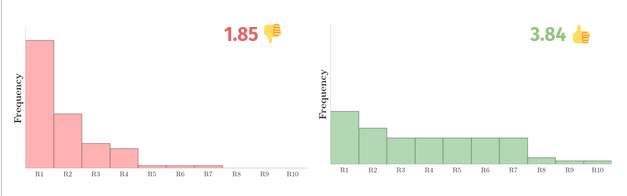
\includegraphics[width=0.6\textwidth]{img/temp/ar_example.png}
    \caption{Example of AR metric.}
    \label{fig:ar_example}
\end{figure}

Another metric we use for comparing the tokenizers is Average Rank (AR). The motivation for this metric is that we want to measure how many tokens are effectively used in the vocabulary for representing the corpus. Each language will have some amount of tokens dedicated to it in the vocabulary and our goal is to measure this allocation. We also want to take into account how frequently are these tokens used. We hypothesize that very frequent and very rare tokens are not as useful for the language models as the high-frequency tokens might be too ambiguous and low-frequency tokens might not have enough training examples to learn from \cite{gowda_finding_2020}. We therefore propose to measure the average rank (the position of the token sorted by frequency) of tokens \tomaszrep{needed to cover a monolingual corpus, weighted by their probability.}{in the empirical probability distribution over a monolingual corpus.}
% Here one metric suggestion could be something along the lines of "number of tokens from vocabulary of $\tau$ needed to cover the 95/98/100\% of the corpus". That metric would work but the downside is that we do not know how to set the threshold. Moreover we would like the metric to reflect the shape of the distribution of the token coverage. We prefer a distribution that is more balanced. High-frequency tokens might be too ambiguous and low-frequency tokens might not have enough training examples to learn from \cite{gowda_finding_2020}. Therefore we propose a different metric that reflects both the vocabulary allocation and the uniformity of the token distribution. On top of that it is parameter-free.

Given a tokenizer $\tau$ and a language corpus $C_l$, we first tokenize the corpus using the tokenizer $\tau$. Then we compute the empirical probability of the tokens in the tokenized corpus.

\begin{equation}
    \hat{p}_{\tau(C_l)}(t) = \frac{count(t, \tau(C_l))}{\sum_{t' \in \tau(C_l)} count(t', \tau(C_l))}
\end{equation}

We sort the tokens by their probability and assign them ranks from 1 to $|V_\tau|$. The average rank is then the weighted average of the ranks of the tokens, where the weights are the probabilites of the tokens:

\begin{equation}
    AR(\tau, C_l) = \sum_{t \in V_\tau} rank(t, \tau(C_l)) \cdot \hat{p}_{\tau(C_l)}(t)
\end{equation}

The metric is illustrated in Figure \ref{fig:ar_example}. Higher AR signals that the vocabulary contains higher number of tokens used for tokenizing given language. Moreover with high AR we can expect that the tokens are distributed more uniformly.

\tomasz{I suggest creating a subsection here:}
Now, we would like to address how our \textit{average rank} compares to different metrics used in the literature. 

First, we examine the \textit{average log probability} (ALP) defined in \citet{zheng_allocating_2021}. This metric is proposed for the same purpose as our AR metric. It is also said to measure language-specific vocabulary capacity and the authors claim that it is "penalized by the subword units with low-frequency". Surprisingly, we can show that the ALP metric is equivalent to the product of negative entropy and average tokenized length.

Given a monolingual corpus composed of sentences $C_l = {s_1, ..., s_{|C_l|}}$ from the language $l$ and tokenized with $\tau$, the ALP is defined as follows \cite{zheng_allocating_2021}:

\begin{equation}
\label{eq:alp}
    ALP(\tau, C_l) = \frac{1}{|C_l|} \sum_{s \in C_l} \sum_{t \in s} \log p(t)
\end{equation}

Where $p(t) = \frac{\mathrm{cnt}(t)}{\sum_{t' \in V_\tau} \mathrm{cnt}(t')}$ is the empirical probability of token $t$ in the corpus $C_l$. 

% In plain words, we sum the log probabilities of all tokens in the corpus and divide by the number of sentences in the corpus.

We can simplify the formula \autoref{eq:alp} by observing that we add up the log token probabilities $\log p(t)$ repeatedly by summing over all sentences and all tokens in sentences. Consequently, the sum can be simply expressed in terms of token occurrence multiplied by the log token probability. We denote $V_\tau$ the set of all tokens in the tokenizer vocabulary $\tau$ and $\mathrm{cnt}(t)$ the number of occurrences of token $t$ in the corpus $C_l$. We can rewrite the ALP metric as follows:

\begin{equation}
    ALP(\tau, C_l) = \frac{1}{|C_l|} \sum_{t \in V_\tau} \mathrm{cnt}(t) \log p(t)
\end{equation}

From here we can derive the relationship between token length (\autoref{eq:tl_def}), information entropy and ALP metric as follows:

\begin{align}
ALP(\tau, C_l) &= \frac{1}{|C_l|} \sum_{t \in V_\tau} \mathrm{cnt}(t) \log p(t) \\
&= \frac{1}{|C_l|} \sum_{t \in V_\tau} \frac{\sum_{t' \in V_\tau} \mathrm{cnt}(t')}{\sum_{t' \in V_\tau} \mathrm{cnt}(t')} \mathrm{cnt}(t) \log p(t) \\
&= \frac{\sum_{t' \in V_\tau} \mathrm{cnt}(t')}{|C_l|} \sum_{t \in V_\tau} \frac{\mathrm{cnt}(t)}{\sum_{t' \in V_\tau} \mathrm{cnt}(t')} \log p(t) \\
&= \frac{\sum_{t' \in V_\tau} \mathrm{cnt}(t')}{|C_l|} \sum_{t \in V_\tau} p(t) \log p(t) \\
&= \frac{\sum_{s \in C_l}|\tau(s)|}{|C_l|} \sum_{t \in V_\tau} p(t) \log p(t) \label{eq:alp_entropy_last_step}\\
&= TL(\tau, C_l) \cdot (- H(p))
\end{align}

In step \ref{eq:alp_entropy_last_step} we express the total number of tokens in corpus $C_l$ by counting over all sentences $s \in C_l$ and summing the number of tokens in each sentence $|\tau(s)|$.

% By analysis of ALP we see that the metric is composed of two metrics that are already well defined. Strangely, the metrics are multiplied together even though the effects of the metrics go against each other. On one hand the lower the token length the better (lower tokenized sentence length means longer and more meaningful tokens), on the other hand arguably, the higher entropy the better (more uniform distribution is better than very unbalanced distribution). It is not clear why would we want to multiply these two metrics together. The authors do not provide this analysis and discussion. \xxx{now interpretaion occured to me: the best ALP is achieved when we have short tokens that are balanced. So actually it could be interesting. But still the authors do not provide this analysis.}

By examination of ALP, it becomes evident that the metric is a composition of two already well-established metrics. Interestingly, these metrics are multiplied together, even though they seem to be inversely related. On the one hand, shorter token lengths are generally considered to be better (as a shorter tokenized sentence length means longer and more meaningful tokens), while on the other, a higher entropy is often deemed more desirable (a more uniform distribution is preferable to a more skewed one). One interpretation could be that high ALP is achieved when the vocabulary consists of a large number of short tokens that are similarly useful (have a uniform distribution). The authors, unfortunately, do not provide an analysis or discussion to shed light on this aspect. \xxx{We also note that the two metrics have different units, if we would want to combine them, it would be useful to add some factor that would determine which of the two metrics we deem more important.}

In comparison to our average rank, ALP measures the number of used tokens and the uniformity of the distribution thanks to the entropy in the equation. On the other hand, the ALP metric is punished by the length of the tokens, which is counterintuitive. We therefore stick to our AR metric, which is more intuitive and does not suffer from this issue.


\subsubsection{Average rank and entropy}

Next, a natural question is what is the difference between average rank and information entropy. The entropy of the tokenized corpus is defined as follows:

\begin{equation}
    H(\tau, C_l) = - \sum_{t \in V_\tau} p(t) \log p(t)
\end{equation}

Recall that we define average rank as follows:

\begin{equation}
    AR(\tau, C_l) = \sum_{t \in V_\tau} rank(t) \cdot p(t)
\end{equation}

We see that entropy provides similar characteristics as AR in the sense that more uniform distributions result in higher entropy and more tokens dedicated to a language also result in higher entropy. As we can see, the formula for entropy and AR differ only in the sign and one of the multiplied terms. The sign is not important as we are only interested in the relative values of the metrics. The difference in the multiplied terms is that AR uses the rank of the token, while entropy uses the log probability of the token. 

To proceed with the analysis, we will assume that the tokens follow Zipf's distribution. This is a reasonable assumption for natural language data. The Zipf's distribution is defined as follows:

\begin{equation}
    p_{zipf}(t) = \frac{1}{rank(t) \cdot H_{|V_\tau|}}
\end{equation}

Where $H_{|V_\tau|}$ is the $|V_\tau|$-th harmonic number used as a normalization constant.

Taking the logarithm of $p_{zipf}(t)$, we get:

\begin{equation}
    \log p_{zipf}(t) = - \log rank(t) - \log H_{|V_\tau|}
\end{equation}

Now if we plug in the log probability of the token into the entropy formula and leave out the constant as we are interested only in the relative values with a fixed vocabulary size, we get:

\begin{equation}
    H(\tau, C_l) \propto \sum_{t \in V_\tau} p(t) \log rank(t)
\end{equation}

We see that under the Zipfian assumption, the entropy may be viewed as an "average log rank". We empirically check this by computing average rank, average log rank, and entropy the Figure \ref{fig:ar_alr_entropy}.

\begin{figure}
    \centering
    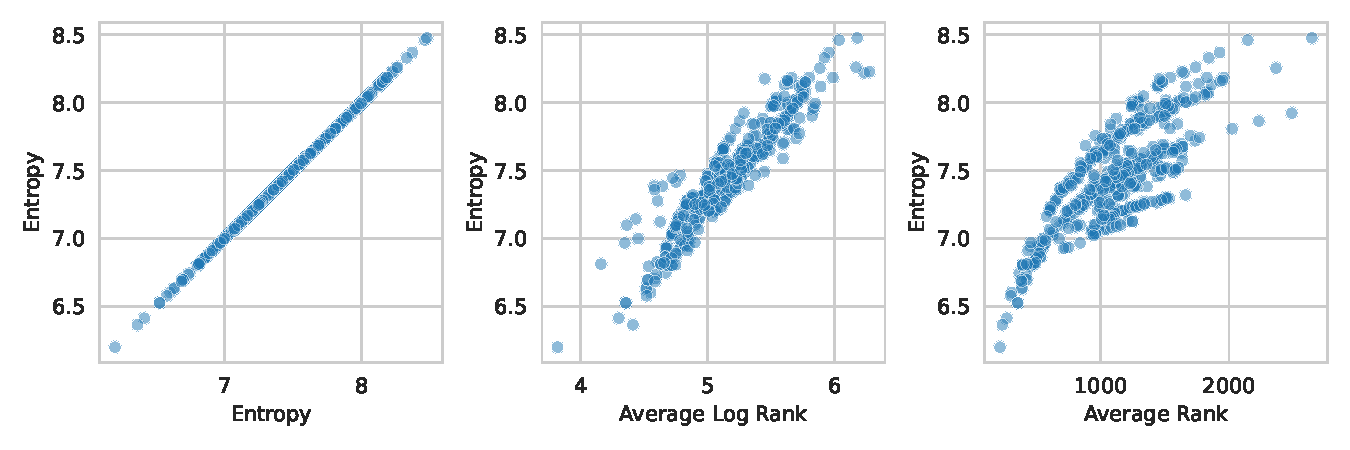
\includegraphics[width=0.9\textwidth]{figures/ar_alr_entropy.pdf}
    \caption{We compute the average rank, average log rank, and entropy for different tokenizers and languages. Then we plot each metric against entropy. We see that entropy and average log rank are similar, which supports our assumption that the tokens follow Zipf's distribution.}
    \label{fig:ar_alr_entropy}
\end{figure}

This provides us with an intuitive understanding of the difference between the two metrics. AR and entropy can be viewed as being related, with the difference being in their sensitivity to the rank of the tokens. AR, being directly related to rank, is more sensitive to changes in probability in lower-frequency tokens. This is because the weighted average used in AR is more affected by linear rank values than the logarithmic rank values used in entropy calculation.

\subsection{Jensen-Shannon Divergence}
\label{sec:jsd}

\begin{figure}[h]
    \centering
    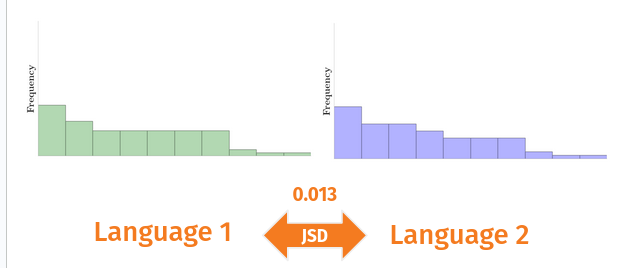
\includegraphics[width=0.5\textwidth]{img/temp/jsd_example.png}
    \caption{Jensen-Shannon Divergence \tomasz{cite the source: poster}}
    \label{fig:jsd_example}
\end{figure}

The Jensen-Shannon Divergence (JSD) is a metric that measures the similarity between two probability distributions. It is defined as follows:

\begin{equation}
    JSD(p, q) = \frac{1}{2} \cdot (KL(p||m) + KL(q||m))
\end{equation}

Where $m = \frac{1}{2} \cdot (p + q)$ is the midpoint distribution and $KL(p||q)$ is the Kullback-Leibler divergence. 

\begin{equation}
    KL(p||q) = \sum_{t \in V_\tau} p(t) \log \frac{p(t)}{q(t)}
\end{equation}

We will use JSD for the analysis of an overlap between two languages given a tokenizer. Tokenization of two monolingual corpora $C_{l_1}$ and $C_{l_2}$ with the same tokenizer $\tau$ will result in two probability distributions over the vocabulary $V_\tau$. We will denote these distributions as $\hat{p}_{\tau(C_{l_1})}$ and $\hat{p}_{\tau(C_{l_2})}$. 

Computing the JSD between the two distributions will result in a metric that measures how much the two distributions overlap. The JSD is a symmetric metric that is bounded between 0 and 1. Low JSD means that the two distributions are similar, high JSD means that the two distributions are different. 

Overlap in tokenization has been studied in \citet{wu_beto_2019}, although the metric used there was the absolute number of overlapping tokens. The benefit of using Jensen-Shannon divergence for measuring the vocabulary overlap is that the metric takes into account the occurrence of the shared tokens. This is important because some of the overlapping tokens may be for example infrequent emojis or other special tokens that do not carry much information about the language nor the actual overlap in more meaningful tokens.

\citet{chung_improving_2020} uses the Wasserstein distance (or the "earth mover's distance") to measure the overlap between two languages. We believe this is \tomaszrep{a mistake}{suboptimal} as the Wasserstein distance is defined for probability measures (probability distributions on a given metric space). The tokenizer vocabulary has no metric structure and the authors of the article do not specify how they define the metric on the vocabulary. It is therefore not suitable to use the Wasserstein distance for measuring the overlap between two tokenizers.

\subsection{Alphabet size and out-of-vocabulary tokens}

Among the metrics we propose, we also measure the alphabet size of the tokenizers defined as the number of tokens of length 1 in the vocabulary:

\begin{equation}
    \mathrm{Alphabet} = |\{t \in V_\tau, |t| = 1\}|
\end{equation}

We also measure the number of out-of-vocabulary (OOV) tokens in the corpus. The UNK token is a special token that used to represent all the tokens that are not present in the vocabulary $V_\tau$. We measure the number of UNK tokens in the corpus as follows:

\begin{equation}
    \mathrm{OOV} = \sum_{t \in \tau(C_l)} \mathbbm{1}_{t = \mathrm{<UNK>}}
\end{equation}

Where $\mathbbm{1}_{t = \mathrm{<UNK>}}$ is an indicator function that is 1 if the token is UNK and 0 otherwise. Because we use the same validation set for all the tokenizers, we can compare the number of OOV tokens directly between the tokenizers. Note that in the literature, the out-of-vocabulary tokens are measured as a OOV rate (number of OOV tokens divided by the total number of tokens in the corpus). We do not use this metric because the values of the OOV rate are small for the subword tokenizers and therefore slightly harder to compare.
\tomasz{I think OOV rate could be better because it's not sensitive to the size of the corpus. But if you already compute the abs. number then leave it.}

% Further, we will be mainly concerned with the tokenization of the training corpora $\tau(C_l)$ and the empirical distribution over the tokenizer vocabulary:

% \xxx{fix the equation once I settle on the notation. The denominator is wrong here}

% - test the tokenizer metrics, show correlation between CPT, AR and JSD -> downstream
%     - define the metricshe implementation}

% In \cite{limisiewicz_tokenization_2023} we have compared the Unigram LM and BPE tokenizers. We have found that generally, the BPE tokenizer performs better on the tokenizer intrinsic metrics and the downstream tasks. During the work on the thesis we have found that this finding might have been heavily influenced by the choice of the implementation of the Unigram LM training algorithm. In \cite{limisiewicz_tokenization_2023} we have used the Huggingface implementation of the tokenizers. In the later experiments we have used the Sentencepiece implementation. We have found that the Sentencepiece implementation produces tokenizers that close the gap in the intrinsic evaluation. We have therefore decided to use the Sentencepiece implementation for all experiments in this thesis.

% \xxx{add image}

% \xxx{TODO: add the other factors - co
%         - CPT
%         - AR
%         - JSD
%     - compare 4 tokenizers
%         - vanilla Unigram, vanilla BPE
%         - NoOverlap - to study the effect of the overlap
%         - TokMix - to ensure a uniform 
%     - experiments for 6 languages
%     - experiments for 20 languages

% \section{Investigating the influence of the tokenizer on the language model}

\section{Evaluation procedures}

In this section, we introduce the evaluation procedures that we use to evaluate the tokenizers. We first describe the types of experiments we do with the tokenizers. Then we explain the intrinsic evaluation procedure. Then we describe the extrinsic evaluation procedure.

\subsection{Types of experiments}

Generally, we can distinguish two types of experiments we do with the tokenizers we compare in this thesis. The first type of experiment is comparing different tokenizers to each other using the evaluation metrics we introduced in the previous section. For example, we can compare the Unigram LM tokenizer to the BPE tokenizer. To do this, we will train the tokenizers on the same training corpus and then evaluate them using the intrinsic evaluation metrics on validation sets \tomaszrep{from}{for} all the languages $L$. 

The second type of experiment is comparing different tokenizers on downstream tasks. For example, we can compare the Unigram LM tokenizer to the BPE tokenizer on the task of natural language understanding. To do this, we will train the tokenizers on the same training corpus and then use the tokenizers to train otherwise identical language models. Then we will evaluate the language models on \tomaszrep{the same validation sets from}{test[?] sets for} all the languages $L$. 

\subsection{Intrinsic evaluation}
\label{sec:intrinsic_evaluation}

For the intrinsic evaluation of a set of tokenizers, we compute the metrics we introduced in the previous section on the validation sets from all the languages $L$. We compute the metrics for each tokenizer and validation language separately. Then, we compare the per language metrics between the tokenizers. Because the metrics are generally different for different languages (for example the characters per token for Chinese will be always smaller than the characters per token for English), we will compare the relative differences between the tokenizers rather than the absolute values.

We will also compute the overall metrics for the whole set of languages $L$. We do this by averaging the metrics over all the languages. We use the macro average over languages, which means that we average the metrics for each language with the same weight. We use the macro average because we want to assess equally the \tomaszrep{improvements over}{impact on} the high-resource and low-resource languages. This is a choice we make to assess each language equally. Different weighting schemes might be more appropriate for different applications. Equal weighting across languages is also in line with how are multilingual models evaluated in the related work \cite{ruder_xtreme-r_2021}.

The JSD metric which measures the \textit{vocabulary overlap} is defined between a pair of languages, measuring the overlap between the two. We compute the overall overlap by considering the JSD values for all pairs \tomasz{of languages:} $l_1, l_2 \in L, l_1 \neq l_2$.

\subsection{Extrinsic evaluation}
\label{sec:extrinsic_evaluation}
%     - extrinsic evaluation
%         - in-language / cross-language
%             - overall - why macroaverage, per-language, how to do per-language in cross-lingual where there are pairs (we focus on target results)
%             - seeds, averaging, bootstrapping
            %     - on how to compute significance for the cross-lingual tasks
            %         - we want to compare the average over languages
            %         - we can use bootstrapping to compute the confidence intervals
            %             - for each language select a random seed and compute the average over these seeds
            %             - sample many times and compute the confidence intervals
%         - probing vs finetuningn
%             - vysvětlit proč jsou všechny experimenty probing a jak se to liší a proč jsme to vybrali
%         - tasks NLI, NER, POS tagging, ...
%     - correlation between intrinsic and extrinsic
%         - how to compute the correlation
%         - míra korelace závisí na tom, jak moc se liší experimenty. Když porovnáváme jen stejné experimenty, pak nám vyjde nízká

For the extrinsic evaluation of \tomaszrep{a set of}{} tokenizers, we compare the performance of \tomaszrep{a set of}{corresponding} language models that differ only in the tokenizers used.
\tomasz{The performance is compared}{We evaluate the performance} on a set of language understanding tasks.
Because the language models are identical except for the tokenizer used, the differences in the performance will be caused only by the differences in the tokenizers and random factors such as the weight initialization of the language models.

Concretely, given a set of tokenizers, we train \tomaszrep{a set of}{corresponding} masked language models with the same architecture and pretraining data.
 We then evaluate the models by training linear classifiers (probes) on top of the contextualized word embeddings produced by the language models. 
 For a given pretrained model, we train probes for each task-language combination utilizing training data in all languages given for the task.
 For each configuration, we train 3 random initializations of the probe with different seeds to acquire more stable results and an estimate of the variation. In total, $N_\mathrm{models} \times N_\mathrm{tasks} \times N_\mathrm{languages} \times N_\mathrm{seeds}$ probes are trained to compare the performance of the models for one experiment.

We use probing \cite{conneau_what_2018,belinkov_interpretability_2020,blevins_analyzing_2022} to evaluate the language modeling capability of the models. Instead of finetuning we freeze the base model and train only linear classifiers on top of the outputs of the base model. This approach allows us to evaluate the language modeling capability of the models without the influence of the finetuning procedure. 
\tomaszrep{We choose probing because it leads to less noisy results than finetuning.}{[I'm afraid it's false]}

% the noise could be caused by the smaller difference between pretraining data amount and the amount of data used for finetuning.

To evaluate a model $m$ on task $t$ and languages $t_L$, we will train probes $f_{m, t, l_\mathrm{src}}$ for each training (source) language $l_\mathrm{src} \in t_L$. Then the probe will be evaluated on the task test sets in languages $l_\mathrm{tgt} \in t_L$ using standard classification metric \tomaszrep{s used for the given task such as accuracy and the F1 score.}{ (in our case: accuracy or F1).} 
% full probe notation: $f_{m, t, l_\mathrm{src}}: \mathbb{R}^d \rightarrow \mathcal{D}_t$

% given model outputs $\vec{x} \in $, we can evaluate the performance of the probe on a given language $l_\mathrm{tgt}$ by computing the accuracy of the probe on the test set for the given language $l_\mathrm{tgt}$.

\subsubsection{Evaluation schemes}

We will distinguish between two evaluation schemes - in-language evaluation and cross-language \xxx{(cross-lingual?)} evaluation. 

The in-language performance of the model $m$ for task $t$ and a language $l$ will be computed by evaluating the probe $f_{m, t, l}$ on the test set for the same language $l$. 
The overall in-language performance of the model $m$ for task $t$ will be computed by averaging the in-language performance over all the languages $l \in t_L$. 

The cross-language performance of the model for task $t$ from the source language $l_\mathrm{src}$ to the target language $l_\mathrm{tgt}$ will be computed by evaluating the probe $f_{m, t, l_\mathrm{src}}$ on the test set for a different language $l_\mathrm{tgt} \neq l_\mathrm{src}$. 
The overall cross-language performance of the model $m$ for task $t$ will be computed by averaging the cross-language performance over all the language pairs $l_\mathrm{src}, l_\mathrm{tgt} \in t_L, l_\mathrm{src} \neq l_\mathrm{tgt}$.
Moreover, we will compute the cross-language performance per language $l$ of the model $m$ for task $t$ by averaging the cross-language performance over all the languages $l_\mathrm{src} \in t_L$ given a target language $l$.

When considering the results per language in both evaluation schemes, it is useful to consider only the relative differences between the models rather than absolute values. The performance of the models for a given language is influenced by eg. by the amount of training data available for the language. Therefore, when interpreting the results per language, we will choose a reference model and compute the relative difference between the performance of the reference model and the other models.

\subsubsection{Correlation between intrinsic and extrinsic evaluation}
\label{sec:correlation_intrinsic_extrinsic}

To support the claim that intrinsic evaluation is a good proxy for extrinsic evaluation, we will compute the correlation between intrinsic and extrinsic evaluation. Because the tokenizer metrics and model performance are influenced by the evaluation language as mentioned in the previous paragraph and in \autoref{sec:intrinsic_evaluation}, we center the tokenizer metrics and downstream task results by subtracting the mean for each language in the in-language setting or pair of languages in the cross-lingual setting. In both cases, means are computed across all tokenizers. We present Spearman’s correlation coefficient and the associated p-value.

\subsubsection{Variation estimation}

To account for the inherent randomness of the training procedure, we will train multiple probes for each configuration $(m, t, l)$. We will use 3 random seeds for each probe and report the average performance over the seeds. We will also report the standard deviation of the performance over the seeds. In the case of the summarized performances, we estimate the standard deviation using bootstrapping over the seeds.

Note that because for one tokenizer we pretrain only one model, as it is the most costly part of the experiment, we do not estimate the variance for the pretraining of the model.
\tomaszrep{We will interpret the results of the experiments with this fact in mind.}{[unnecessary]}


% For evaluating the language modeling capability of the models we use two techniques. First, we want to evaluate the performance of the models using finetuning on language understanding tasks. This approach is taken by the related work and it is the standard way of multilingual model evaluation. We use part of the XTREME benchmark, namely the Natural language inference, Part of Speech tagging and Named entity recognition tasks. For each task we finetune on every language and measure the performance on the development set. We do not apply any hyperparameter search apart from choosing a satisfactory learning rate and batch size for each task by running few short experiments. 

% Second, we also use probing \cite{conneau_what_2018,belinkov_interpretability_2020,blevins_analyzing_2022} to evaluate the language modeling capability of the models. We use the same tasks from XTREME benchmark, but instead of finetuning we freeze the base model and train only simple linear classifiers on top of the base model. This approach allows us to evaluate the language modeling capability of the models without the influence of the finetuning procedure. 


% \tomasz{Here, I would write section Extrinsic Evaluation. 
% With general description assesing tokenizer influnce on downstream tasks.
% Details should be provided in the next chapter: Experiments...}


\section{Evaluation on downstream tasks}

Here we present the downstream tasks we use in our paper \cite{limisiewicz_tokenization_2023}. For our further experiments, we use a subset of these tasks (POS, NER, NLI) that we have found to have different responses to the changes in the CPT, AR and JSD metrics.

\subsection{POS}

We use Part of Speech annotations from Universal Dependencies \cite{nivre_universal_2020}. The dataset is available for 17 languages analyzed by us (not covered: Swahili, Thai, Georgian). \tomasz{PROBLEM: You haven't introduced the list of languages yet!} Each word is assigned one of the 17 coarse POS tags.

\subsection{NER}

We use Wikiann dataset \cite{pan_cross-lingual_2017} consisting of Wikipedia articles with annotated named entities of three types: location, person, and organization in IOB2. Following XTREME, we use balanced data splits from \cite{rahimi_massively_2019}.

\subsection{Dependency labeling}

As in Part of Speech, we use Universal Dependencies \cite{nivre_universal_2020} for the dependency relation annotations. We use the largest UD treebank available for each language.
For each word, we predict one of the 37 universal relations to its head word. Because the relation is between two words, we use the concatenation of the two word representations along with their element-wise product as an input to the probe ($[h_{w1}; h_{w2}; h_{w1} \odot h_{w2}]$).

\subsection{NLI}

We use XNLI dataset \cite{conneau_xnli_2018} for Natural Language Inference. We train the linear classification probe on top of the concatenation of two sentence vectors and their element-wise product: $[h_{s1}; h_{s2}; h_{s1} \odot h_{s2}]$. We predict one of two relations between the first of sentences (called premise): contradicts, entails, or is neutral to the second sentence (called a hypothesis). We evaluate XNLI with the accuracy of classification.

XNLI contains data for 15 languages (not covered: te, ta, mr, he, ka).

\subsection{Sentence Retrieval}
We use up to 1,000 sentences aligned for pairs of languages from Tatoeba dataset \cite{artetxe_massively_2019}. For the pairs including English, we use the same sample as in XTREME data collection. For other pairs, we perform sampling ourselves. 

We compute the cosine similarity between sentence representations across languages and find the best alignment with the Hungarian algorithm\cite{kuhn_hungarian_1955}. We compute the accuracy as the number of correctly aligned sentences divided by the total number of sentences.


\section{Implementation Details}
\tomasz{IMO good place to dump all Appendi-worthy details.}

\subsection{Tokenizers}
\subsection{Model Pretraining}
\subsection{Probing}


\section{Reproducing the vocabulary balancing methods}
\label{sec:reproducing_the_vocabulary_balancing_methods}
% - replication of the previous balancing work
%     - the code is not available for Chung and Liang, for Zheng we reimplement even though the code is available
%     - therefore we follow all papers closely
%     - Chung
%         - reproductions of chung are available in the paper Overlap-based Vocabulary Generation Improves Cross-lingual Transfer Among Related Languages
%             - they do not replicate the results of Chung
%         - we run training with 8k vocab size, unigram, coverage 0.9995 (default in Sentencepiece) for each language
%             - this is specified in the paper
%             - we use 1M lines for each language which we have shown to be enough in preliminary experiments
%         - we compute the binary vectors for each language and normalize them to unit length
%         - we compute clusters using k-means, with k=4, 8, 12, 16, 20 (=all languages)
%         - train the tokenizers on the clusters
%             - target vocab size is 120k, again use Sentencepiece defaults
%             - to reach the vocab size we train also +10\%, +20\%, +30\% of the target size and then prune
%         - then we merge the tokenizers

%     - Liang
%         - we follow the same procedure as in Chung
%         - compute negative log-likelihoods for each token over the corpus and use the euclidean distance to compute the similarity
%         - but we use the sizes from Zheng

In this section, we describe our reproduction of the existing methods for balancing the low- and high- resource languages in the vocabulary. As the code for two out of three of the methods is not available, we follow and reimplement the original papers closely and describe the differences in our implementation.

The methods of \citet{chung_improving_2020} and \citet{liang_xlm-v_2023} follow a three step process: 1) grouping the languages into clusters by similarity, 2) running the Unigram LM tokenizer training on the clustered corpora and 3) combining the cluster-vocabularies into a single, multilingual vocabulary. Because of their similarity, we refer to the two as the clustering methods. The method of \citet{zheng_allocating_2021} works in two steps: 1) training the Unigram LM tokenizers for each language separately and 2) selecting the best vocabulary size for each language and combining the vocabularies into a single, multilingual vocabulary.

As we can see the methods share the last merging step and differ in the clustering approaches. We therefore describe the clustering approaches first, then we describe the Zheng method and finally we describe the merging step common for all methods.

\subsection{Reproducing the clustering methods}
% \tomasz{General remark: It's better to keep experiments definition (i.e. hypothesis statement and experiment overview.) separated from implementation details.
% The later are important bu shouldn't steal attention of the reader from the story.}

The first step for the Chung and Liang methods is to train monolingual Unigram LM tokenizers for each language $l$ from the set of 20 languages $L$. As specified in \citet{chung_improving_2020}, we use the default Sentencepiece settings. Namely, we use the Unigram LM model, character coverage of 99.95\%, number of seed sentencepieces is 1M. \xxx{add all parameters to appendix?}. 
For training the monolingual tokenizers, we use 1M lines for each language which we have shown to be enough in preliminary experiments \autoref{sec:data_size}. This choice also corresponds to the \citet{zheng_allocating_2021} method, which uses 1M lines for each language. The vocabulary size differs between Chung and Liang and so we train two sets of monolingual tokenizers, with 8k and 30k vocabulary sizes respectively.

We arrive at $|L|$ vocabularies $V^l$. Next, we take the union of all vocabularies $V^L = \bigcup_{l \in L} V^l$ and compute the "vector representation" $\vec{v}^l$ for each language $l$ as described in \autoref{sec:chung} and \autoref{sec:liang}. For Chung, we compute a binary vector of size $|V^L|$, where each element $\vec{v}^l_i$ is 1 if the token $i$ is in the vocabulary $V^l$ of language $l$ and 0 otherwise. For Liang, we compute a vector of size $|V^L|$, where each element $\vec{v}^l_i$ is the negative log-likelihood of the token $i$ in the language $l$ as computed by the Sentencepiece training algorithm. We set the log-likelihood of the tokens not in the vocabulary to 0 as inferred from the Figure 1 in \cite{liang_xlm-v_2023}. We discuss this choice in more detail in the discussion \autoref{sec:language_vectors}.

With the vector representations $\vec{v}^l$ we can cluster the languages into $k$ clusters $C^k$ using the k-means algorithm. We use the implementation from \texttt{scikit-learn} \cite{pedregosa_scikit-learn_2011} with the default parameters. \citet{chung_improving_2020} reports using the cosine distance for the k-means algorithm. We normalize the language representation vectors to unit length, to achieve the same effect. In the case of Liang, we stick to Euclidean distance as the authors do not mention using a different metric. We experiment with $k \in \{4, 8, 16, 20\}$. Note that $k=20$ corresponds to separating each language into a separate cluster which is similar to the method \textsc{TokMix} we introduce in \citet{limisiewicz_tokenization_2023} and \citet{zheng_allocating_2021} we replicate next.

Then, given a clustering of languages $C$, for each cluster $c_j \in C$ we create a new training corpus by concatenating all of the CC100 data belonging to the cluster\footnote{Because of computational constraints, we cap the total number of lines per cluster to 20M. If the cluster corpus exceeds the total number of lines, we subsample the available data with $\alpha=1.0$}. We run the Sentencepiece algorithm again on these clustered corpora to arrive at cluster-specific vocabularies $V^{c_j}$. The vocabulary size for each cluster is determined following the Chung and Liang methods. For both methods, we want to arrive at the final size of 120k tokens after merging the cluster-specific vocabularies. Therefore we need to determine the size of each cluster vocabulary $|V^{c_j}|$ such that $\sum_{j=1}^k |V^{c_j}| = 120k$. The Chung method sets the size of the cluster vocabulary to be proportional to the size of the union over the monolingual vocabularies $|\bigcup_{l \in c_j} V^l|$ to determine the size of each cluster vocabulary as follows:

\begin{equation}
    |V^{c_j}| = \frac{|\bigcup_{l \in c_j} V^l|}{\sum_{i=1}^k |\bigcup_{l' \in c_i} V^{l'}|} \cdot 120k
\end{equation}

The Liang method proposes to set the size of the cluster vocabulary to be proportional to the sum of the vocabulary allocations from \citet{zheng_allocating_2021} for the languages belonging to the cluster. We use the allocations we reproduce in \autoref{subsec:reproducing_vocap}.
\footnote{
    Here we slightly improve the methods of Chung and Liang. By following the original method as described above, the final size of the vocabulary will be lower than the target we set. This is because the cluster vocabularies $V^{c_j}$ will contain overlapping tokens and merging will remove these duplicates. This negative effect becomes larger with the increasing number of clusters $k$. Therefore, on top of training the prescribed cluster vocabulary of size $|V^{c_j}|$, we also train slightly larger vocabularies $V_q^{c_j'}$ of size $|V_q^{c_j}| = q|V^{c_j}|$ for $q = 1.1, 1.2, 1.3$. We then select the minimum $q$ that results in a vocabulary size of at least 120k tokens after merging the cluster vocabularies. After that, we trim the vocabulary if needed. This improvement is done to ensure the final vocabulary size is exactly 120k tokens and the comparison between the methods is fair.
}

After the tokenizers are trained, we merge the vocabularies using the method described in \autoref{subsec:merging_tokenizers}. 

The resulting clusters and the corresponding per-cluster vocabulary sizes are found in Tables \ref{fig:cluster_assignments_k4}, \ref{fig:cluster_assignments_k8}, \ref{fig:cluster_assignments_k16}, and \ref{fig:cluster_assignments_k20}.

\begin{figure}[p]
    \centering
    
    \begin{subtable}{0.49\textwidth}
        \centering
        % ---
        \begin{tabular}{lr}
            \toprule
            Languages & Size \\
            \midrule
            zh, ar, ru, bg & 27425 \\
            el, ur, ta, te, th, he, ka & 48841 \\
            en, es, tr, sw, vi, fr, de & 43622 \\
            hi, mr & 12108 \\
            \bottomrule
        \end{tabular}
        % ---
        \caption{\citet{chung_improving_2020}}
        \label{tab:chung_clusters_k4}
        

    \end{subtable}
    \hfill
    \begin{subtable}{0.49\textwidth}
        \centering
        % ---
        \begin{tabular}{lr}
        \toprule
        Languages & Size \\
        \midrule
        el, zh, ar, ur, ta, te, th, he, ka & 61285 \\
        en, es, tr, sw, vi, fr, de & 43370 \\
        hi, mr & 10370 \\
        ru, bg & 16970 \\
        \bottomrule
        \end{tabular}
        % ---
        \caption{\citet{liang_xlm-v_2023}}
        \label{tab:liang_clusters_k4}
    \end{subtable}

    \caption{Cluster assignments for 4 clusters}
    \label{fig:cluster_assignments_k4}
\end{figure}

\begin{figure}[p]
    \centering
    
    \begin{subtable}{0.49\textwidth}
        \centering
        % ---
        \begin{tabular}{lr}
            \toprule
            Languages & Size \\
            \midrule
            el & 7458 \\
            ru, bg & 12975 \\
            ta, te & 14318 \\
            en, es, tr, sw, th, ka, vi, fr, de & 56509 \\
            ar, ur & 13788 \\
            hi, mr & 12030 \\
            zh & 7458 \\
            he & 7458 \\
            \bottomrule
            \end{tabular}
        % ---
        \caption{\citet{chung_improving_2020}}
        \label{tab:chung_clusters_k8}
        

    \end{subtable}
    \hfill
    \begin{subtable}{0.49\textwidth}
        \centering
        % ---
        \begin{tabular}{lr}
            \toprule
            Languages & Size \\
            \midrule
            en, fr & 12256 \\
            es, tr, sw, de & 27342 \\
            ru, bg & 16970 \\
            ar, ur & 12256 \\
            vi & 3770 \\
            hi, mr & 10370 \\
            el, ta, te, th, he, ka & 37713 \\
            zh & 11313 \\
            \bottomrule
        \end{tabular}
        % ---
        \caption{\citet{liang_xlm-v_2023}}
        \label{tab:liang_clusters_k8}
    \end{subtable}

    \caption{Cluster assignments for 8 clusters}
    \label{fig:cluster_assignments_k8}
\end{figure}

\begin{figure}[p]
    \centering
    
    \begin{subtable}{0.49\textwidth}
        \centering
        % ---
        \begin{tabular}{lrlr}
            \toprule
            Langs. & Size & Langs. & Size \\
            \midrule
            ar, ur & 14020 & zh & 7582 \\
            tr & 7582 & he & 7582 \\
            en, fr & 13549 & ta & 7582 \\
            hi, mr & 12232 & sw & 7582 \\
            ru, bg & 13194 & ka & 7582 \\
            vi & 7582 & th & 7582 \\
            te & 7582 & es & 7582 \\
            el & 7582 & de & 7582 \\
            \bottomrule
        \end{tabular}
        % ---
        \caption{\citet{chung_improving_2020}}
        \label{tab:chung_clusters_k16}
        

    \end{subtable}
    \hfill
    \begin{subtable}{0.49\textwidth}
        \centering
        % ---
        \begin{tabular}{lrlr}
            \toprule
            Langs. & Size & Langs. & Size \\
            \midrule
            de & 8228 & te & 7200 \\
            ar & 7200 & vi & 4113 \\
            en, fr & 13370 & el & 10285 \\
            hi, mr & 11313 & ta & 4113 \\
            ru, bg & 18513 & zh & 12342 \\
            ka & 8228 & sw & 6170 \\
            he & 5142 & es & 7200 \\
            tr, th & 14400 & ur & 6170 \\
            \bottomrule
        \end{tabular}
        % ---
        \caption{\citet{liang_xlm-v_2023}}
        \label{tab:liang_clusters_k16}
    \end{subtable}

    \caption{Cluster assignments for 16 clusters}
    \label{fig:cluster_assignments_k16}
\end{figure}

\begin{figure}[h]
    \centering
    
    \begin{subtable}{0.32\textwidth}
        \centering
        % ---
        \begin{tabular}{lr}
            \toprule
            Languages & Size \\
            \midrule
            ar & 7200 \\
            bg & 7200 \\
            de & 7200 \\
            el & 7200 \\
            en & 7200 \\
            es & 7200 \\
            fr & 7200 \\
            he & 7200 \\
            hi & 7200 \\
            ka & 7200 \\
            mr & 7200 \\
            ru & 7200 \\
            sw & 7200 \\
            ta & 7200 \\
            te & 7200 \\
            th & 7200 \\
            tr & 7200 \\
            ur & 7200 \\
            vi & 7200 \\
            zh & 7200 \\
            \bottomrule
        \end{tabular}
        % ---
        \caption{\citet{chung_improving_2020}}
        \label{tab:chung_clusters_k20}
        

    \end{subtable}
    \hfill
    \begin{subtable}{0.32\textwidth}
        \centering
        % ---
        \begin{tabular}{lr}
            \toprule
            Languages & Size \\
            \midrule
            ar & 7200 \\
            bg & 8228 \\
            de & 8228 \\
            el & 10285 \\
            en & 6170 \\
            es & 7200 \\
            fr & 7200 \\
            he & 5142 \\
            hi & 5142 \\
            ka & 8228 \\
            mr & 6170 \\
            ru & 10285 \\
            sw & 6170 \\
            ta & 4113 \\
            te & 7200 \\
            th & 6170 \\
            tr & 8228 \\
            ur & 6170 \\
            vi & 4113 \\
            zh & 12342 \\
            \bottomrule
        \end{tabular}
        % ---
        \caption{\citet{liang_xlm-v_2023}}
        \label{tab:liang_clusters_k20}
    \end{subtable}
    \hfill
    \begin{subtable}{0.32\textwidth}
        \centering
        % ---
        \begin{tabular}{lr}
            \toprule
            Languages & Size \\
            \midrule
            ar & 7000 \\
            bg & 8000 \\
            de & 8000 \\
            el & 10000 \\
            en & 6000 \\
            es & 7000 \\
            fr & 7000 \\
            he & 5000 \\
            hi & 5000 \\
            ka & 8000 \\
            mr & 6000 \\
            ru & 10000 \\
            sw & 6000 \\
            ta & 4000 \\
            te & 7000 \\
            th & 6000 \\
            tr & 8000 \\
            ur & 6000 \\
            vi & 4000 \\
            zh & 12000 \\
            \bottomrule
        \end{tabular}
        % ---
        \caption{\citet{zheng_allocating_2021}}
        \label{tab:zheng_allocations}
    \end{subtable}


    \caption{Allocated vocabulary sizes for 20 languages}
    \label{fig:cluster_assignments_k20}
\end{figure}
% \begin{table}
\caption{Cluster assignments for {k} clusters.}
\label{tab:chung_clusters_k20}
\begin{tabular}{lr}
\toprule
Languages & Size \\
\midrule
sw & 7200 \\
ka & 7200 \\
hi & 7200 \\
en & 7200 \\
th & 7200 \\
ru & 7200 \\
tr & 7200 \\
el & 7200 \\
he & 7200 \\
ur & 7200 \\
ar & 7200 \\
zh & 7200 \\
te & 7200 \\
es & 7200 \\
de & 7200 \\
fr & 7200 \\
vi & 7200 \\
ta & 7200 \\
mr & 7200 \\
bg & 7200 \\
\bottomrule
\end{tabular}
\end{table}

% \begin{table}
\caption{Cluster assignments for {k} clusters.}
\label{tab:chung_clusters_k16}
\begin{tabular}{lr}
\toprule
Languages & Size \\
\midrule
ar, ur & 14020 \\
tr & 7582 \\
en, fr & 13549 \\
hi, mr & 12232 \\
ru, bg & 13194 \\
vi & 7582 \\
te & 7582 \\
el & 7582 \\
zh & 7582 \\
he & 7582 \\
ta & 7582 \\
sw & 7582 \\
ka & 7582 \\
th & 7582 \\
es & 7582 \\
de & 7582 \\
\bottomrule
\end{tabular}
\end{table}

% \begin{table}
\caption{Cluster assignments for {k} clusters.}
\label{tab:chung_clusters_k8}
\begin{tabular}{lr}
\toprule
Languages & Size \\
\midrule
el & 7458 \\
ru, bg & 12975 \\
ta, te & 14318 \\
en, es, tr, sw, th, ka, vi, fr, de & 56509 \\
ar, ur & 13788 \\
hi, mr & 12030 \\
zh & 7458 \\
he & 7458 \\
\bottomrule
\end{tabular}
\end{table}

% \begin{table}
\caption{Cluster assignments for {k} clusters.}
\label{tab:chung_clusters_k4}
\begin{tabular}{lr}
\toprule
Languages & Size \\
\midrule
zh, ar, ru, bg & 27425 \\
el, ur, ta, te, th, he, ka & 48841 \\
en, es, tr, sw, vi, fr, de & 43622 \\
hi, mr & 12108 \\
\bottomrule
\end{tabular}
\end{table}


% \input{./tables/liang_clusters_k20.tex}
% \input{./tables/liang_clusters_k16.tex}
% \input{./tables/liang_clusters_k8.tex}
% \input{./tables/liang_clusters_k4.tex}

\subsection{Reproducing the \textsc{VoCap} method}
\label{subsec:reproducing_vocap}

%     - Zheng
%         - train monolingual tokenizers for all 20 languages with vocab sizes 1k ... 40k
%         - load a sample of CC100 data for each language (50k lines per language)
%         - tokenize the data with all of the monolingual tokenizers
%         - compute the ALP for each language and vocabulary size
%         - select the best vocabulary size for each language greedily
%         - we also experiment with optimizing CPT instead of ALP
%         - we also experiment with computing the CPT improvement on each merge step instead of precomputing it for all vocab sizes

%         - they have this suspicious plot with ALP with Joint250k, Joint500k and VoCap500k and the differences are too much

From the high level, the \textsc{VoCap} method works by selecting the best vocabulary size for each language and then merging the monolingual vocabularies. The best vocabulary size is determined by maximizing the overall \textit{Average Log Probability} metric defined in \autoref{eq:alp}. 

To replicate the \textsc{VoCap} method, we first need to compute the \textsc{ALP} metric for each language $l$ and each vocabulary size $V \in {1000, ..., 40\,000}$. To that end, we train monolingual tokenizers using Sentencepiece with default settings for all 20 languages with vocabulary sizes from 1k to 40k.\footnote{The more effective way, not discussed by \citet{zheng_allocating_2021}, would be to modify the Sentencepiece unigram trainer code to produce a tokenizer after each prune iteration. That way we would get series of tokenizers with decreasing vocabulary size in one go, instead of running the trainer 40 times. As the computational cost of training the tokenizers is not high for our reduced set of 20 langugaes, we have not implemented this improvement.} We use 1M lines per language for training the monolingual tokenizers again, following \citet{zheng_allocating_2021}. Note that for Chinese the tokenizer vocabulary size starts at 5k due to the large number of unique logograms in the language. 

% reference for 1M lines: https://github.com/bozheng-hit/VoCapXLM/blob/main/train_mono_spm.py#L73

We then load a sample of CC100 data for each language (100k lines per language) and tokenize each monolingual corpus with the respective tokenizers of increasing vocabulary sizes. We are then able to compute the $\mathrm{ALP}(l, V)$ metric for each language $l$ and each vocabulary size $V$.

Now we can proceed to greedily select the best vocabulary sizes. We start with selecting the lowest vocabulary size for each language (1k for all languages except Chinese where we start with 5k). We merge the selected vocabularies of the tokenizers as explained in \autoref{subsec:merging_tokenizers}. Then in each iteration, we check which language would benefit the most from increasing the vocabulary size by 1000. Concretely, we check the increase in ALP for each language and increase the vocabulary size for that language by merging the bigger vocabulary with the total vocabulary. We repeat this process until the total vocabulary size reaches 120k tokens. Any tokens over the limit are removed from the vocabulary.

Contrary to \citet{zheng_allocating_2021}, we do not use the $\beta$ rescaling factor to account for the pretraining corpus size (we describe the $\beta$ parameter in related work \autoref{sec:zheng}). By setting $\beta$ to 0, we want to achieve the best ALP for each language regardless of its corpus size. This is because our goal is to balance the low-resource languages, not necessarily achieve the best performance on the downstream tasks.

The final vocabulary sizes for each language are found in \autoref{tab:zheng_allocations}

% Additionally, we also experiment with optimizing the \textsc{CPT} metric instead of \textsc{ALP}. We also experiment with computing the \textsc{CPT} improvement on each merge step instead of precomputing it for all vocab sizes, since the metric increase might be slightly different for the intermediate tokenizer. None of these modifications lead to substantially better results and so we stick to the original method. \xxx{rewrite this or remove it}

\subsection{Merging the tokenizers}
\label{subsec:merging_tokenizers}

%     - merging the tokenizers
%         - merging is not really described in the papers
%         - of course we take the union of the vocabularies
%         - but how to set the logits?
%             - to illustrate that even this step should be documented, the probabilities of XLM-V vocabulary do not sum to one
%     - reaching the target size
%         - train +10\%, +20\% of the target size and then prune

For all reproduced methods, the last step is to take several Unigram tokenizers and merge them into the final, multilingual tokenizer. Now we will describe how we merge tokenizers in our case. Unfortunately, the merging step is not described fully in any of the reproduced papers. In the case of the Unigram tokenizers, tokenizer $\tau$ consists of vocabulary (set of strings) $V_\tau \subset \Sigma^\star$ and the corresponding logits $L_\tau: \Sigma^\star \rightarrow \mathbb{R}$ so that $\sum_{t \in V_\tau} \exp(L_\tau(t)) = 1$. The logits are used for finding the most probable segmentation of an input sentence. 

To create the merged vocabulary for input tokenizers $\tau_1, ... \tau_m$ we take the union over the vocabularies:

\begin{equation}
    V_\tau \coloneqq \bigcup_{i=1}^m V_{\tau_i}
\end{equation}

We set the merged logits to the log of the average probability of the token in the input tokenizers:

\begin{equation}
    \forall t \in V_\tau: L_\tau(t) \coloneqq \log(\frac{1}{m} \sum_{i}^m \exp(L_{\tau_i}(t)))
\end{equation}

If the token $t$ is not present in some of the input tokenizers, we consider the probability of the token for that tokenizer to be zero. 

In this way the sum of the probabilities of the tokens in the merged vocabulary is one and thus the merged tokenizer is a valid Unigram tokenizer. We can see this by the following derivation. We assume that the input tokenizers $\tau_i$ are valid Unigram tokenizers and thus the sum of the probabilities of the tokens in the input tokenizers is one:

\begin{equation}
\begin{split}
    \sum_{t \in V_\tau} \exp(L_\tau(t)) = \sum_{t \in V_\tau} \exp(\log(\frac{1}{m} \sum_{i}^m \exp(L_{\tau_i}(t)))) = \\
    = \sum_{t \in V_\tau} \frac{1}{m} \sum_{i}^m \exp(L_{\tau_i}(t)) = \frac{1}{m} \sum_{i}^m \sum_{t \in V_\tau} \exp(L_{\tau_i}(t)) = \frac{1}{m} \sum_{i}^m 1 = 1
\end{split}
\end{equation}

% \xxx{the second equality should be maybe more explained}

We argue that this is the most natural way to merge the tokenizers and so we assume this is probably the way the other authors did the merging. By observing the logits in the tokenizer released by \citet{liang_xlm-v_2023}\footnote{\href{https://huggingface.co/facebook/xlm-v-base/blob/main/sentencepiece.bpe.model}{https://huggingface.co/facebook/xlm-v-base/blob/main/sentencepiece.bpe.model}}, we see that the authors do merge the logits in some way but the sum of the probabilities in the final tokenizer is $\approx 4.55$ (not counting the special tokens), which suggests some problems in the merging step. The tokenizer released by \citet{zheng_allocating_2021} seems to be merged correctly\footnote{\href{https://github.com/bozheng-hit/VoCapXLM/blob/main/VoCap\_500k/sentencepiece.bpe.model}{https://github.com/bozheng-hit/VoCapXLM/blob/main/VoCap\_500k/sentencepiece.bpe.model}}.

% \xxx{We have also checked empirically, that the individual tokenizers perform similarly to the merged tokenizer and so the merging procedure seems to preserve the properties of the merged tokenizers.}

% urls for the tokenizers:
% https://github.com/bozheng-hit/VoCapXLM/blob/main/VoCap_500k/sentencepiece.bpe.model
% https://huggingface.co/facebook/xlm-v-base/blob/main/sentencepiece.bpe.model


% \section{Proposed methods}

% - motivation for word-balancing:
%     - we assume that there is a topic imbalance in the CC100 corpus
%         - assume there is 99% of news and 1% biology
%         - the name of the ministry of agriculture will be more common than the word "evolution"
%             - but it is more useful to cover the most common words in biology than the uncommon words in news
%         - by balancing the words we may achieve better coverage of the topics
%     - we assume it is better to split roots of words and not have many inflected forms of the same word
%         - if the word "evolution" occurs much more frequently than "evoluce", the model might learn "evolution" but will oversegment "evoluce"
%         - by balancing the words we may arrive at a better segmentation because it will be more useful to split "evolution" into evolu + tion and evoluce into evolu + ce

% We propose to compare the replicated methods with the original method from \citet{conneau_unsupervised_2020} with $\alpha=0.3$. Moreover, we also propose to simply use the balancing factor $\alpha=0.0$, which leads to data balance, that is equal in the number of lines across all languages. 
% Specifically, both methods use the same Sentencepiece tokenizer implementation as used in the replications. We use the Unigram LM as in \citet{conneau_unsupervised_2020}, set the vocabulary size to 120k and leave the rest of the parameters default. The main difference is the training data where $\alpha=0.0$ uses 1M lines per language and $alpha=0.3$ uses a sample of 10M lines from the CC100 with the language balance factor $\alpha=0.3$. 

% The next method we propose is based 

